\section{Source Code} \label{app:sourcecode}

\textit{Source code} penelitian ini tersedia secara publik pada repositori GitHub berikut:

\begin{table}[H]
\caption{Informasi repositori \textit{source code} penelitian}
\label{tab:app.sourcecode}
\centering
\begingroup
\setlength{\tabcolsep}{6pt}
\renewcommand{\arraystretch}{1.4}
\footnotesize
\begin{tabular}{|>{\raggedright\arraybackslash}p{2.0cm}|>{\raggedright\arraybackslash}p{7.5cm}|}
\hline
\rowcolor{gray!20} \multicolumn{1}{|c|}{\textbf{Atribut}} & \multicolumn{1}{c|}{\textbf{Keterangan}} \\
\hline
\textbf{Platform} & GitHub \\
\hline
\textbf{URL} & \url{https://github.com/Youngstg/SIBI-Classification-VideoMAE} \\
\hline
\textbf{Deskripsi} & Repositori berisi seluruh skrip pelatihan, konfigurasi eksperimen, dan utilitas pemrosesan data untuk klasifikasi gerakan SIBI menggunakan arsitektur VideoMAE. \\
\hline
\end{tabular}
\endgroup
\end{table}

\section{Demo Aplikasi} \label{app:demo}

Demo aplikasi pengenalan bahasa isyarat SIBI berbasis VideoMAE tersedia secara publik pada platform Hugging Face Spaces berikut:

\begin{table}[H]
\caption{Informasi demo aplikasi pengenalan isyarat SIBI}
\label{tab:app.demo}
\centering
\begingroup
\setlength{\tabcolsep}{6pt}
\renewcommand{\arraystretch}{1.4}
\footnotesize
\begin{tabular}{|>{\raggedright\arraybackslash}p{2.0cm}|>{\raggedright\arraybackslash}p{7.5cm}|}
\hline
\rowcolor{gray!20} \multicolumn{1}{|c|}{\textbf{Atribut}} & \multicolumn{1}{c|}{\textbf{Keterangan}} \\
\hline
\textbf{Platform} & Hugging Face Spaces \\
\hline
\textbf{URL} & \url{https://huggingface.co/spaces/Luckystg/SIBI_Recognition_VideoMAE-demo} \\
\hline
\textbf{Deskripsi} & Antarmuka demo interaktif yang memungkinkan pengguna mengunggah klip video isyarat SIBI dan memperoleh hasil klasifikasi secara langsung menggunakan model VideoMAE terbaik (E12). \\
\hline
\end{tabular}
\endgroup
\end{table}

\section{Dataset SIBI} \label{app:dataset}

Dataset SIBI yang digunakan dalam penelitian ini tersedia secara publik pada platform Kaggle berikut:

\begin{table}[H]
\caption{Informasi dataset SIBI}
\label{tab:app.dataset_info}
\centering
\begingroup
\setlength{\tabcolsep}{6pt}
\renewcommand{\arraystretch}{1.4}
\footnotesize
\begin{tabular}{|>{\raggedright\arraybackslash}p{2.0cm}|>{\raggedright\arraybackslash}p{7.5cm}|}
\hline
\rowcolor{gray!20} \multicolumn{1}{|c|}{\textbf{Atribut}} & \multicolumn{1}{c|}{\textbf{Keterangan}} \\
\hline
\textbf{Platform} & Kaggle \\
\hline
\textbf{URL} & \url{https://www.kaggle.com/datasets/luckyimmanuel/sibi-dataset-videomae} \\
\hline
\textbf{Deskripsi} & Dataset terdiri dari 924 klip video untuk 10 kelas kata dasar SIBI, direkam di SLBN PKK Provinsi Lampung dengan proses pemburaman wajah pada seluruh subjek. \\
\hline
\end{tabular}
\endgroup
\end{table}

Tabel~\ref{tab:app.contoh_frame} menampilkan contoh frame representatif dari setiap kelas dataset SIBI setelah proses pemburaman wajah pada subjek.

\begin{table}[H]
\caption{Contoh frame per kelas dataset SIBI setelah pemburaman wajah}
\label{tab:app.contoh_frame}
\centering
\begingroup
\setlength{\tabcolsep}{6pt}
\renewcommand{\arraystretch}{1.4}
\footnotesize
\begin{tabular}{|>{\raggedleft\arraybackslash}p{0.5cm}|>{\raggedright\arraybackslash}p{1.5cm}|>{\centering\arraybackslash}p{2.2cm}|>{\raggedleft\arraybackslash}p{0.5cm}|>{\raggedright\arraybackslash}p{1.5cm}|>{\centering\arraybackslash}p{2.2cm}|}
\hline
\rowcolor{gray!20} \multicolumn{1}{|c|}{\textbf{No}} & \multicolumn{1}{c|}{\textbf{Kelas}} & \multicolumn{1}{c|}{\textbf{Contoh Frame}} & \multicolumn{1}{c|}{\textbf{No}} & \multicolumn{1}{c|}{\textbf{Kelas}} & \multicolumn{1}{c|}{\textbf{Contoh Frame}} \\
\hline
1  & Aku     & \raisebox{-0.35\height}{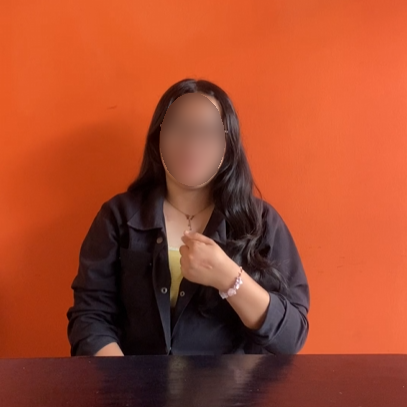
\includegraphics[height=1.45cm,keepaspectratio]{fotoblur_hasil/aku.png}} &
6  & Kamu    & \raisebox{-0.35\height}{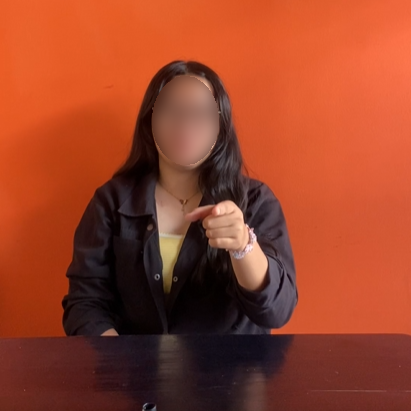
\includegraphics[height=1.45cm,keepaspectratio]{fotoblur_hasil/kamu.png}} \\
\hline
2  & Bapak   & \raisebox{-0.35\height}{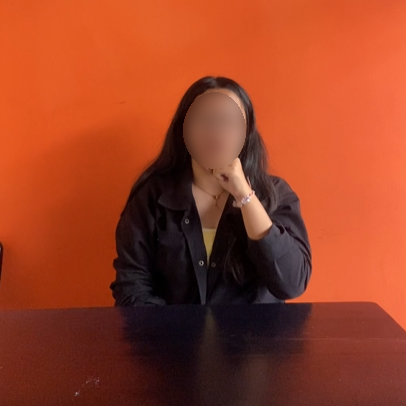
\includegraphics[height=1.45cm,keepaspectratio]{fotoblur_hasil/bapak.png}} &
7  & Mau     & \raisebox{-0.35\height}{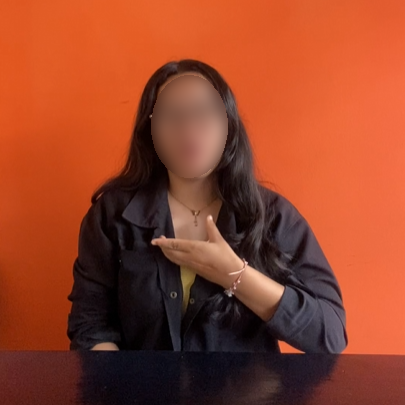
\includegraphics[height=1.45cm,keepaspectratio]{fotoblur_hasil/mau.png}} \\
\hline
3  & Bawa    & \raisebox{-0.35\height}{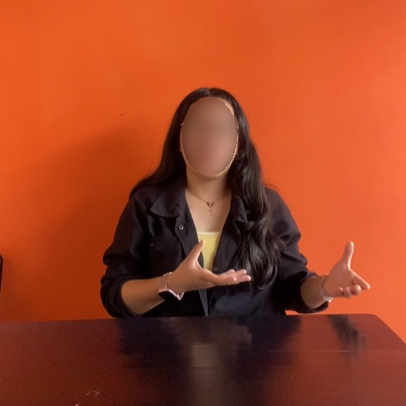
\includegraphics[height=1.45cm,keepaspectratio]{fotoblur_hasil/bawa.png}} &
8  & Pulang  & \raisebox{-0.35\height}{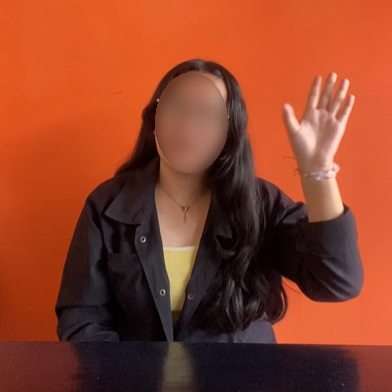
\includegraphics[height=1.45cm,keepaspectratio]{fotoblur_hasil/pulang.png}} \\
\hline
4  & Guru    & \raisebox{-0.35\height}{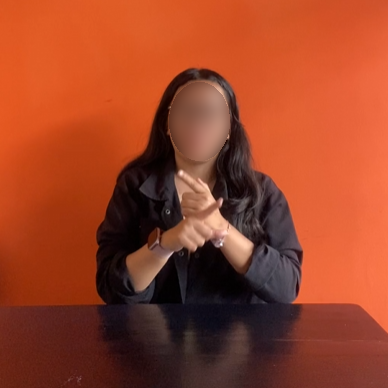
\includegraphics[height=1.45cm,keepaspectratio]{fotoblur_hasil/guru.png}} &
9  & Sekolah & \raisebox{-0.35\height}{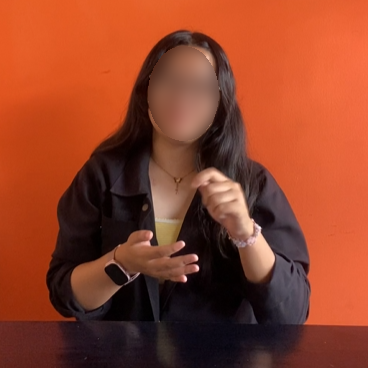
\includegraphics[height=1.45cm,keepaspectratio]{fotoblur_hasil/sekolah.png}} \\
\hline
5  & Ibu     & \raisebox{-0.35\height}{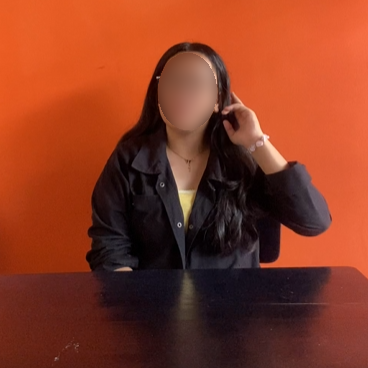
\includegraphics[height=1.45cm,keepaspectratio]{fotoblur_hasil/ibu.png}} &
10 & Suka    & \raisebox{-0.35\height}{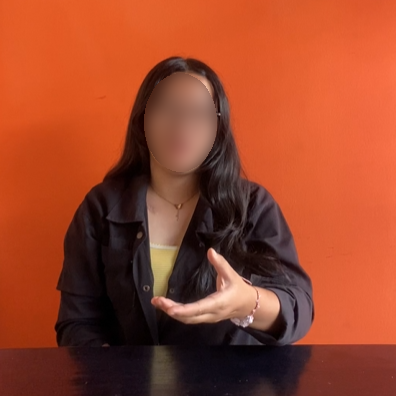
\includegraphics[height=1.45cm,keepaspectratio]{fotoblur_hasil/suka.png}} \\
\hline
\end{tabular}
\endgroup
\end{table}

\section{Dokumentasi Kunjungan SLB PKK Lampung dan Wawancara} \label{app:dokumentasi}
Dokumentasi kunjungan ke SLB PKK Lampung ditunjukkan pada Gambar~\ref{fig:kunjungan-slb}. Foto ini menjadi bukti kegiatan untuk pengumpulan kebutuhan dan verifikasi proses penelitian. Dokumentasi ini juga mencakup hasil wawancara dengan pihak terkait selama penelitian.

\begin{figure}[H]
	\centering
	% 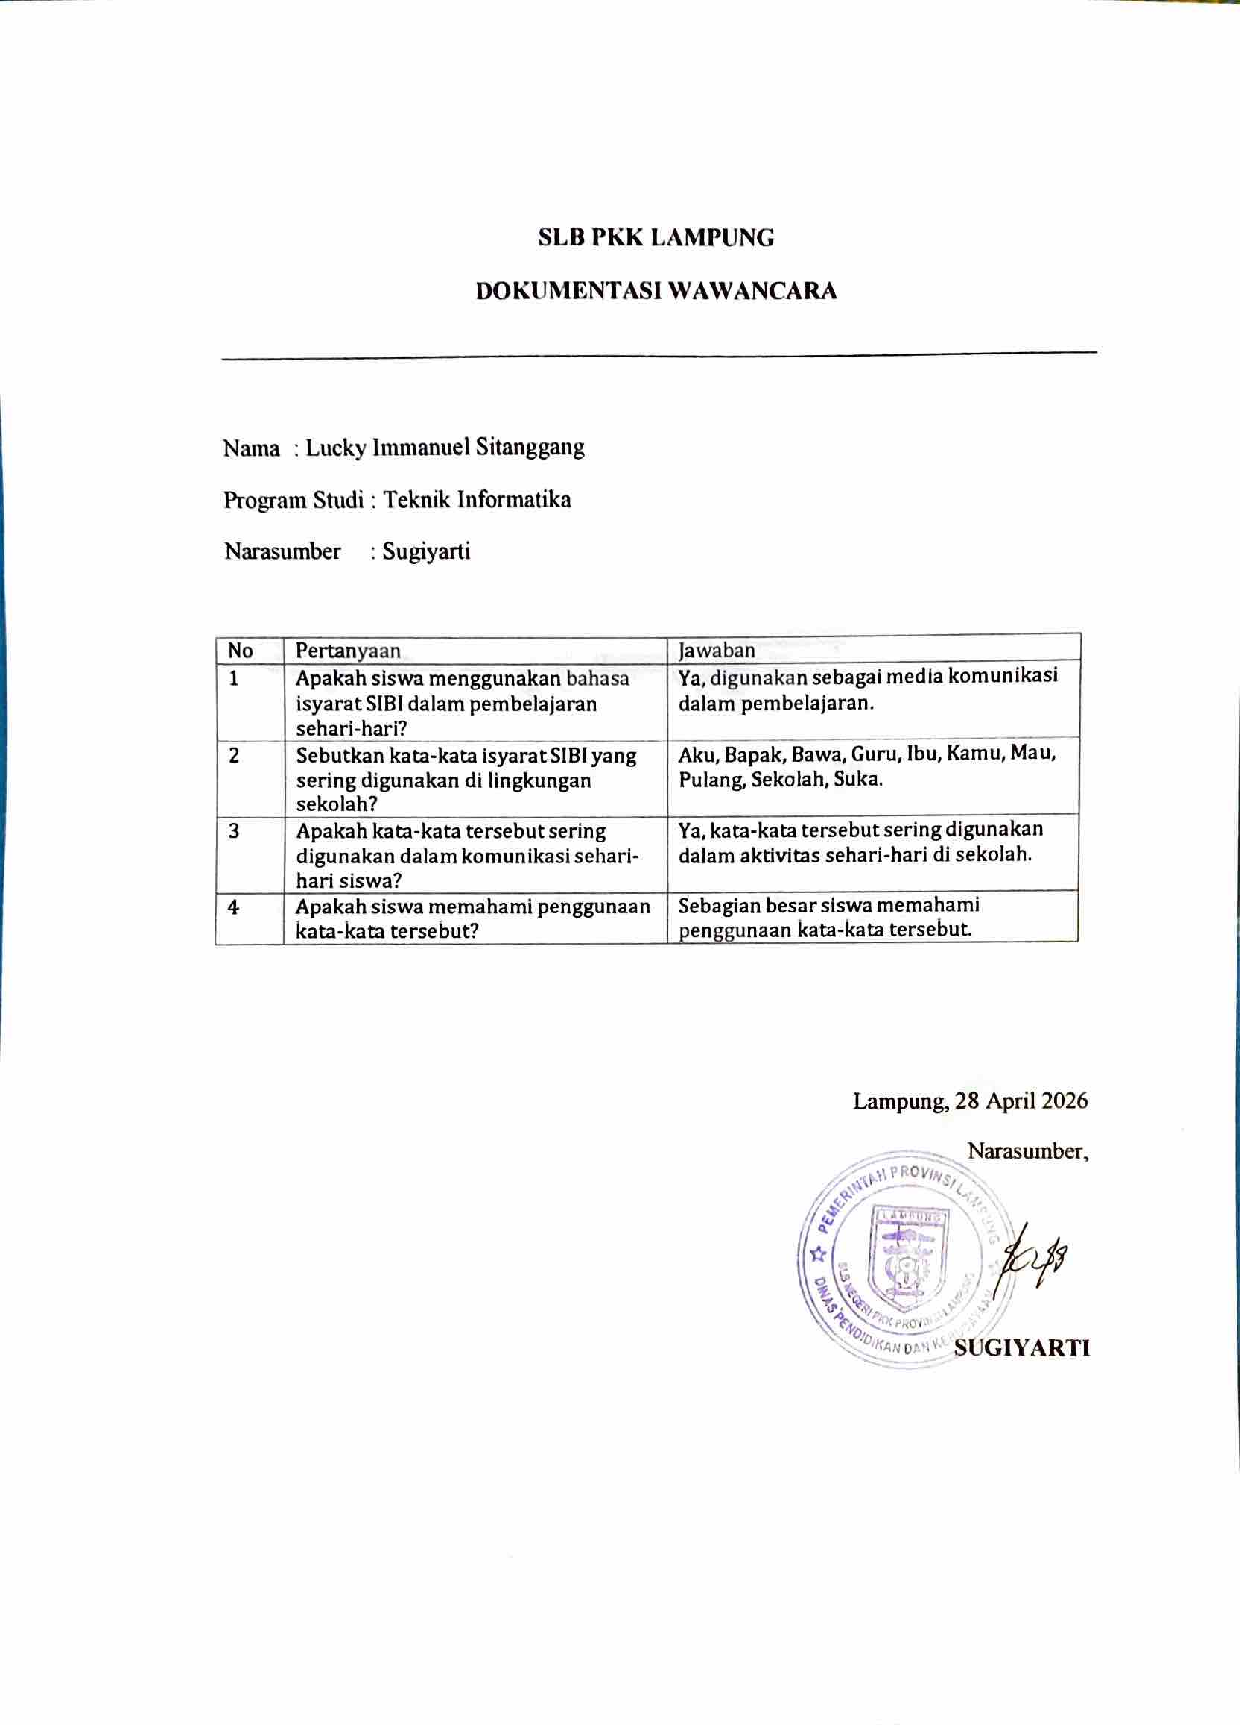
\includegraphics[width=0.9\textwidth]{LAMPIRAN/Dokumenwwc.pdf}
	\caption{Dokumen Wawancara.}
\end{figure}

\begin{figure}[H]
	\centering
	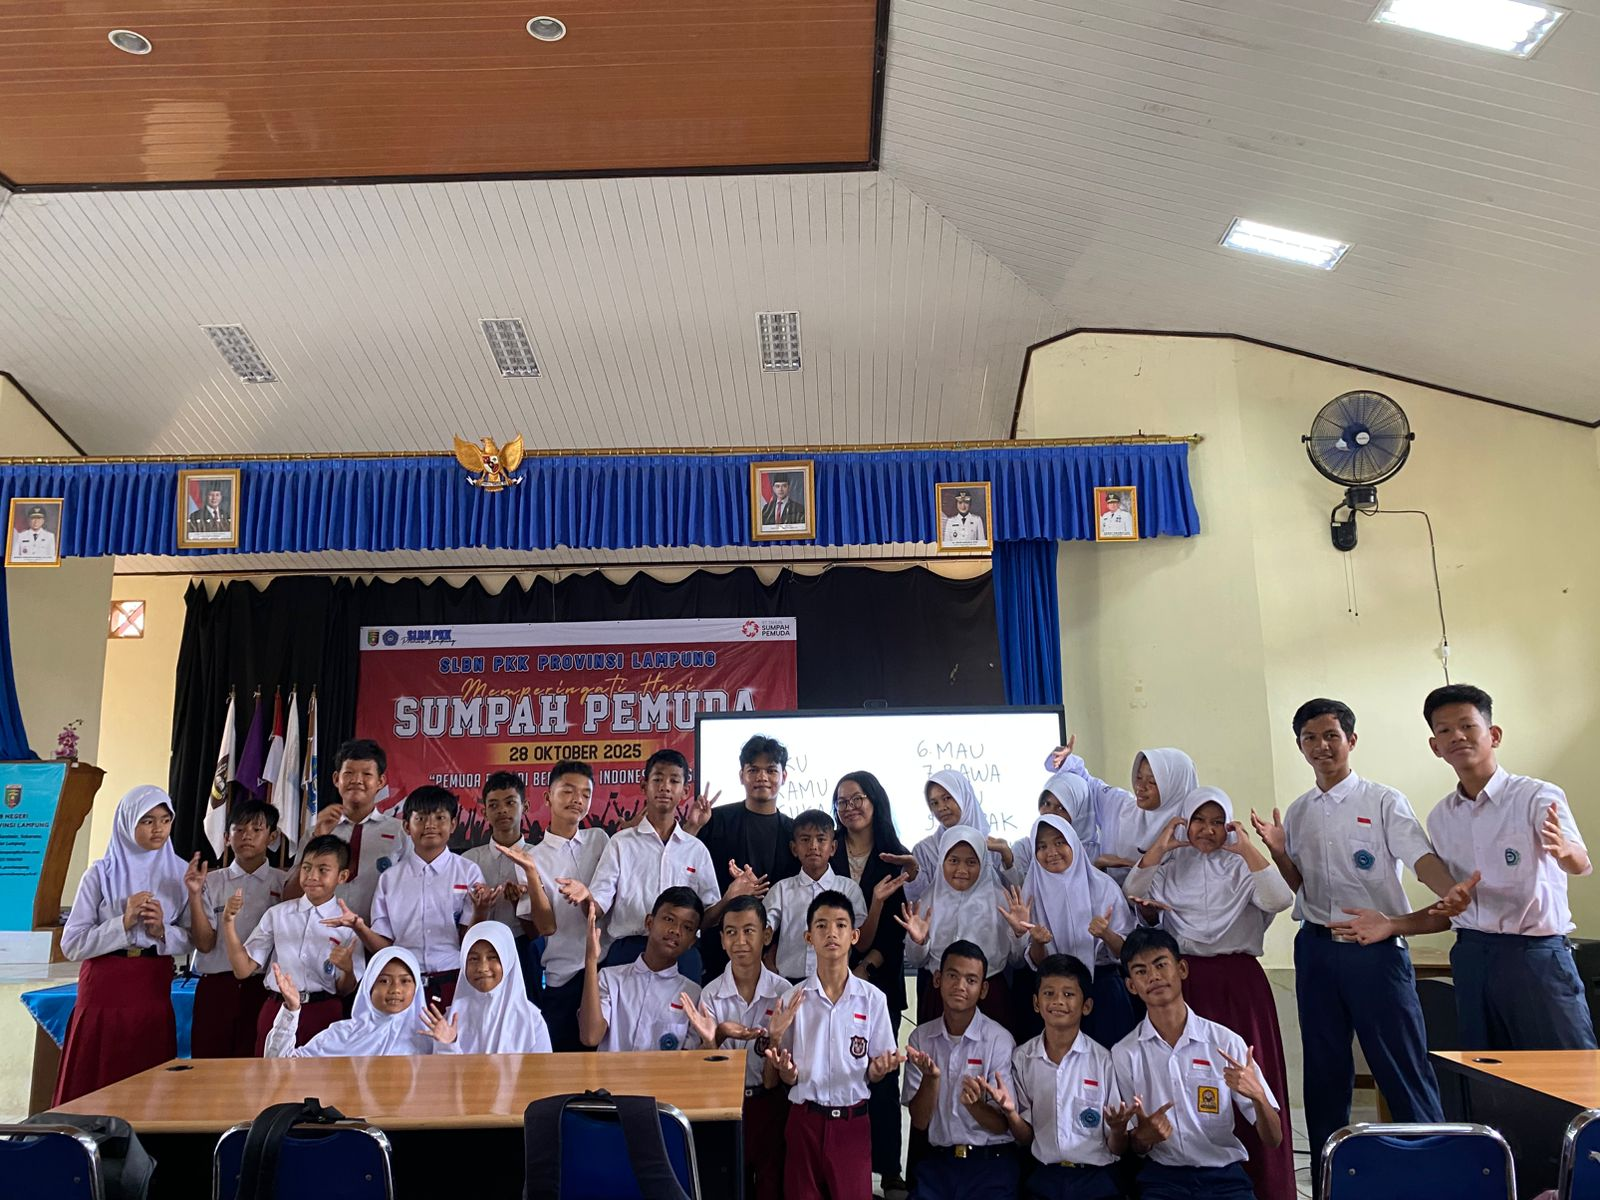
\includegraphics[width=0.9\textwidth]{figure/Gambarkunjungan.jpg}
	\caption{Kunjungan peneliti ke SLB PKK Lampung.}
	\label{fig:kunjungan-slb}
\end{figure}

\section{Surat Persetujuan Data} \label{app:suratpersetujuan}
\begin{figure}[H]
	\centering
	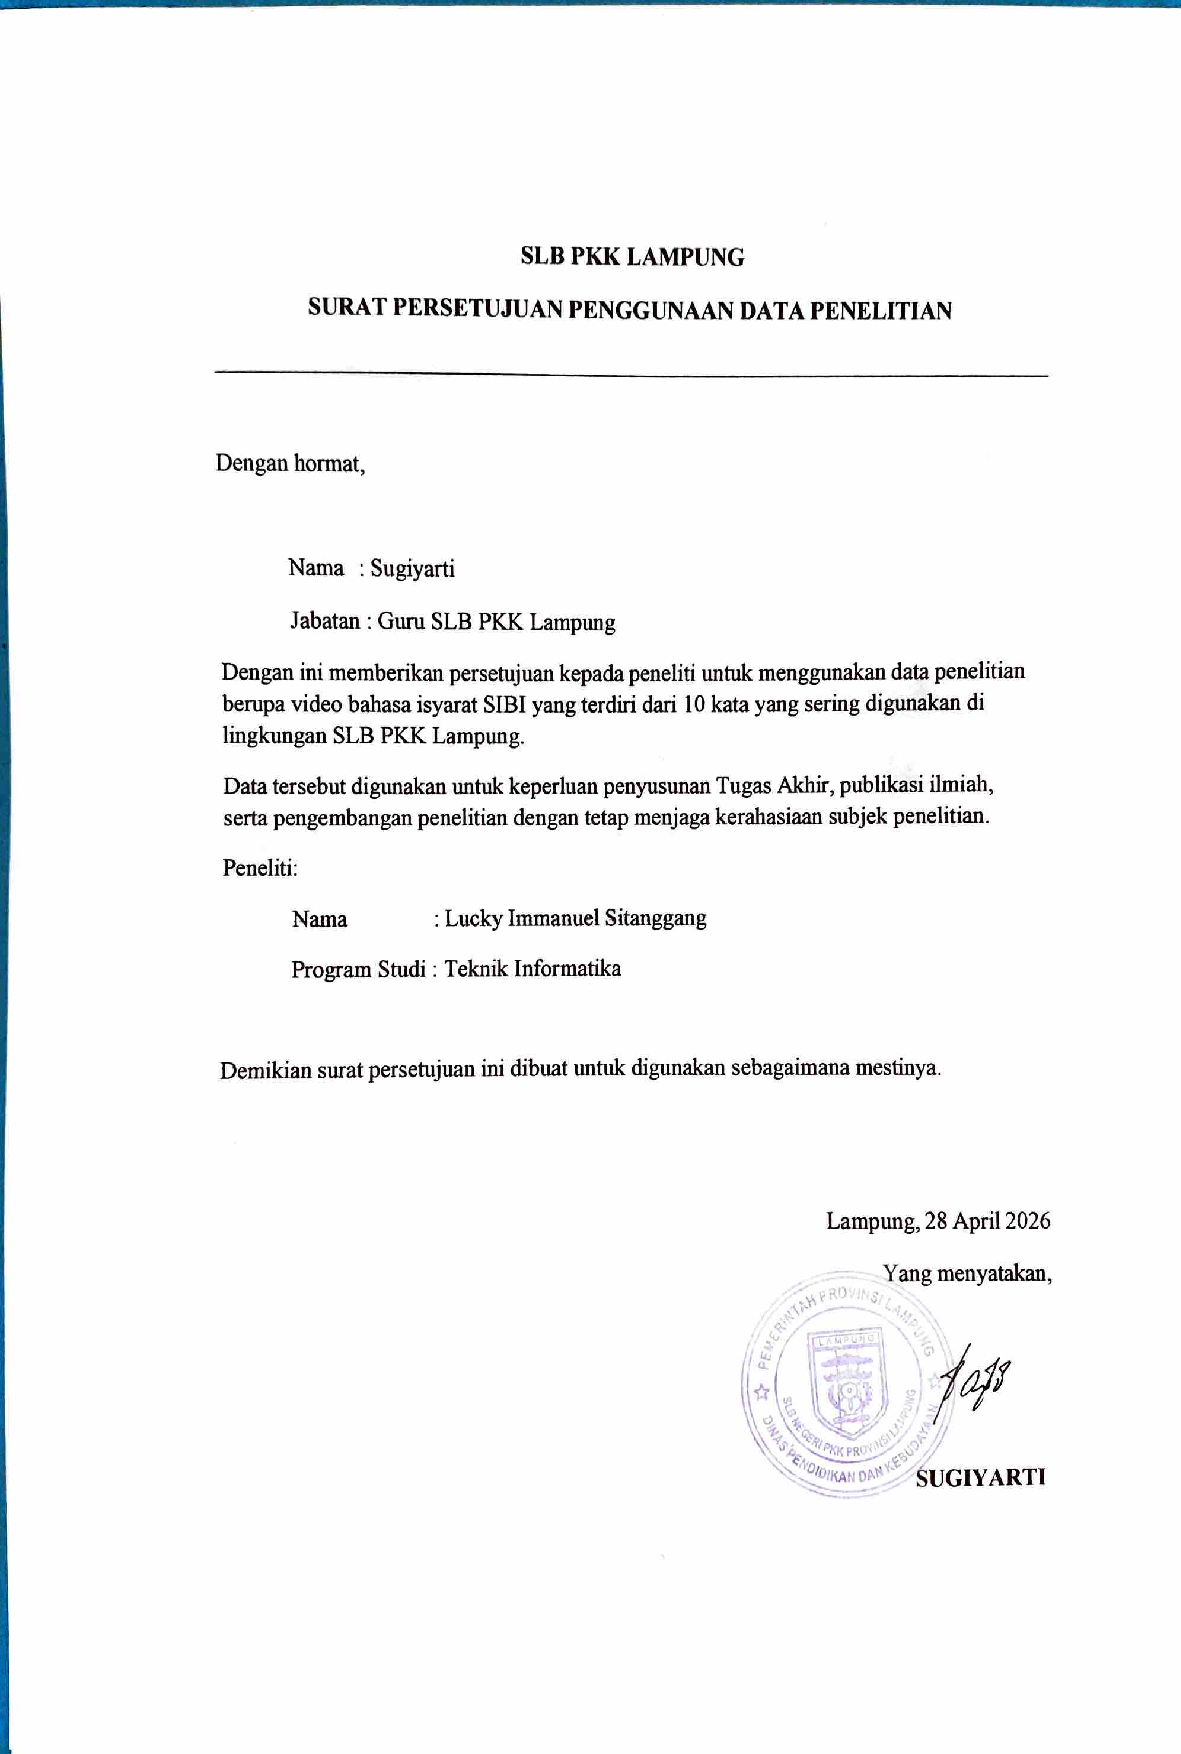
\includegraphics[page=1,width=0.9\textwidth,height=0.82\textheight,keepaspectratio]{LAMPIRAN/SuratPersetujuanData.pdf}
	\caption{Surat persetujuan data penelitian.}
\end{figure}

\section{Surat Validasi Data} \label{app:suratvalidasi}
\begin{figure}[H]
	\centering
	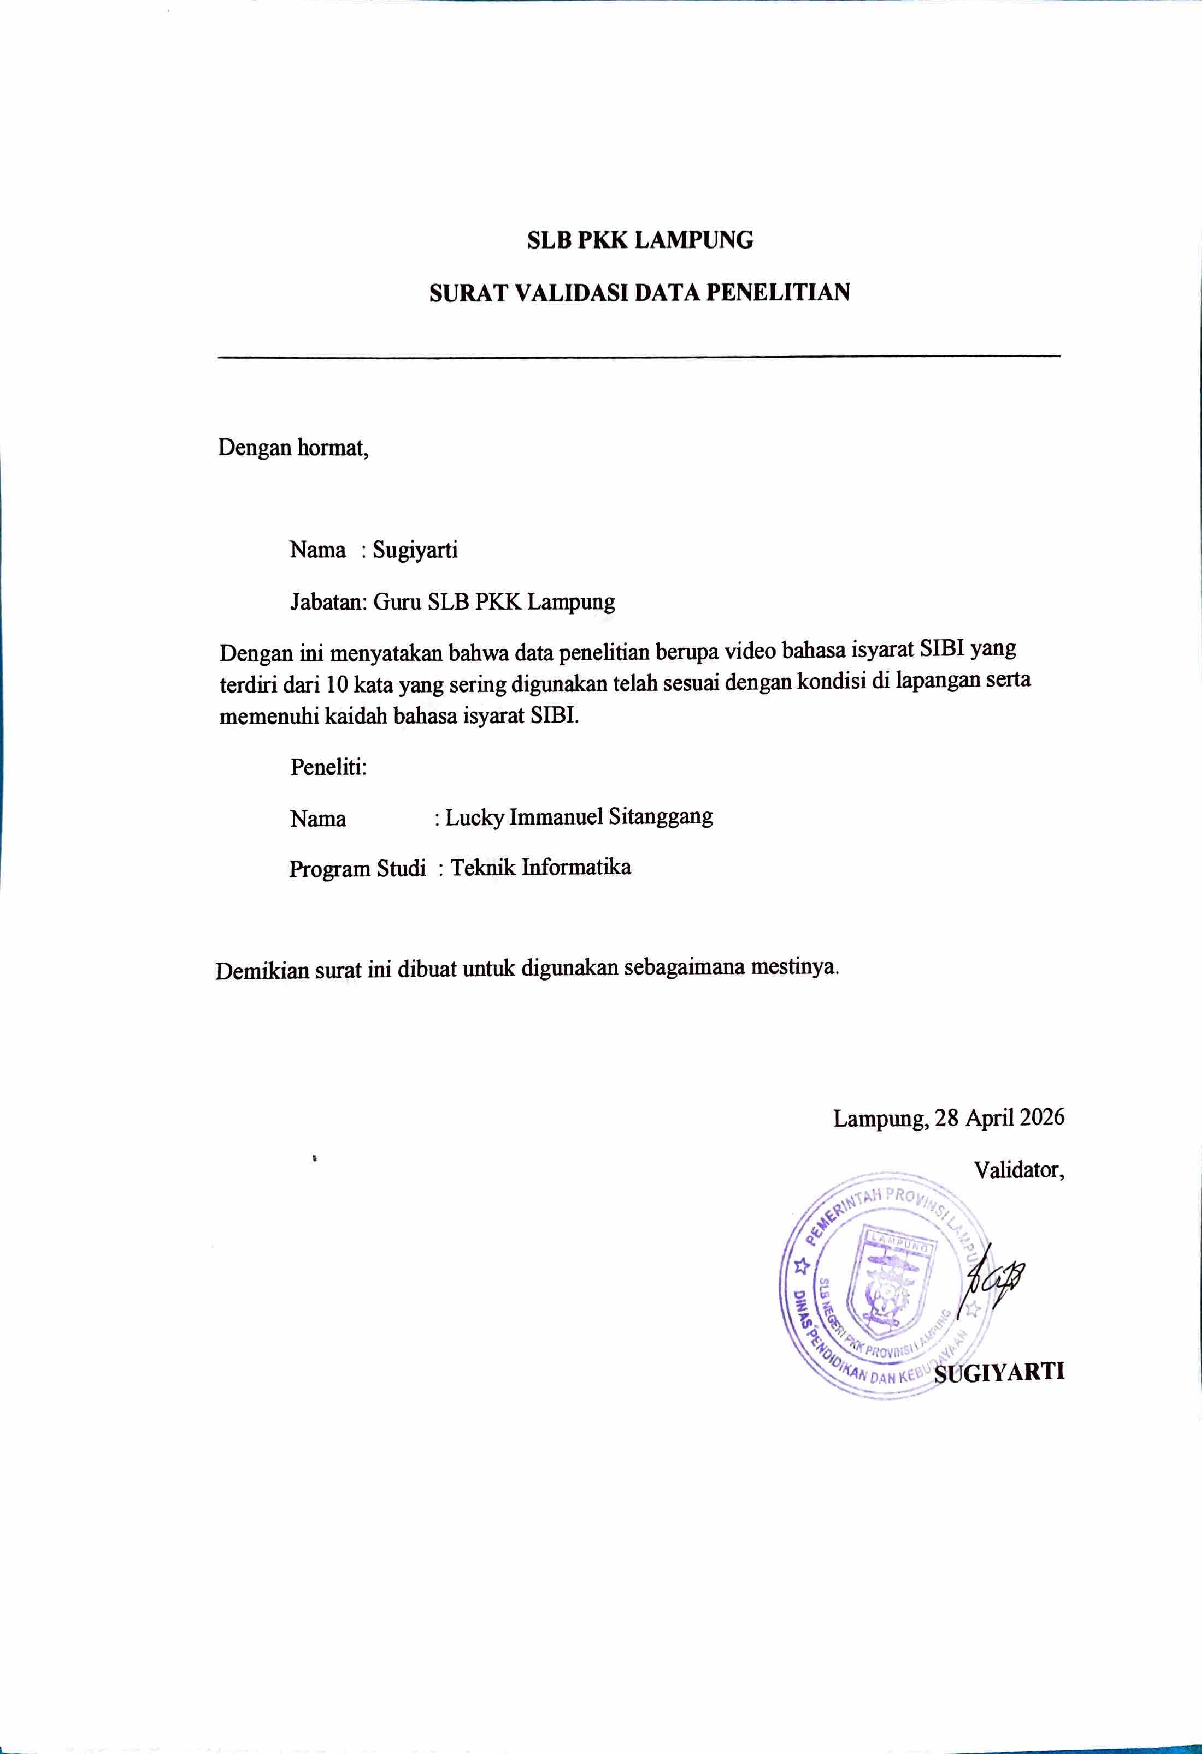
\includegraphics[page=1,width=0.9\textwidth,height=0.82\textheight,keepaspectratio]{LAMPIRAN/SuratValidasiData.pdf}
	\caption{Surat validasi data penelitian.}
\end{figure}
